\section{Passenger density data}
\label{sec:PassengerDensityData}

In order to model the passenger density an understanding of the available data is necessary. In this section the data, visible pattern and other features are discussed.

Figure~\ref{fig:rawData_week} illustrates exemplary the available values of a camera and week. At a more detailed view Figure~\ref{fig:rawData_day} shows the passenger density level of a camera and (week)day. On both Figures, the PdG service times are visible due to the low passenger density level between 01:00 and 05:00 on weekdays.

\begin{figure*}[htbp]

  \centering

  \subfigure[Passenger density distribution of one camera during one week.] {
    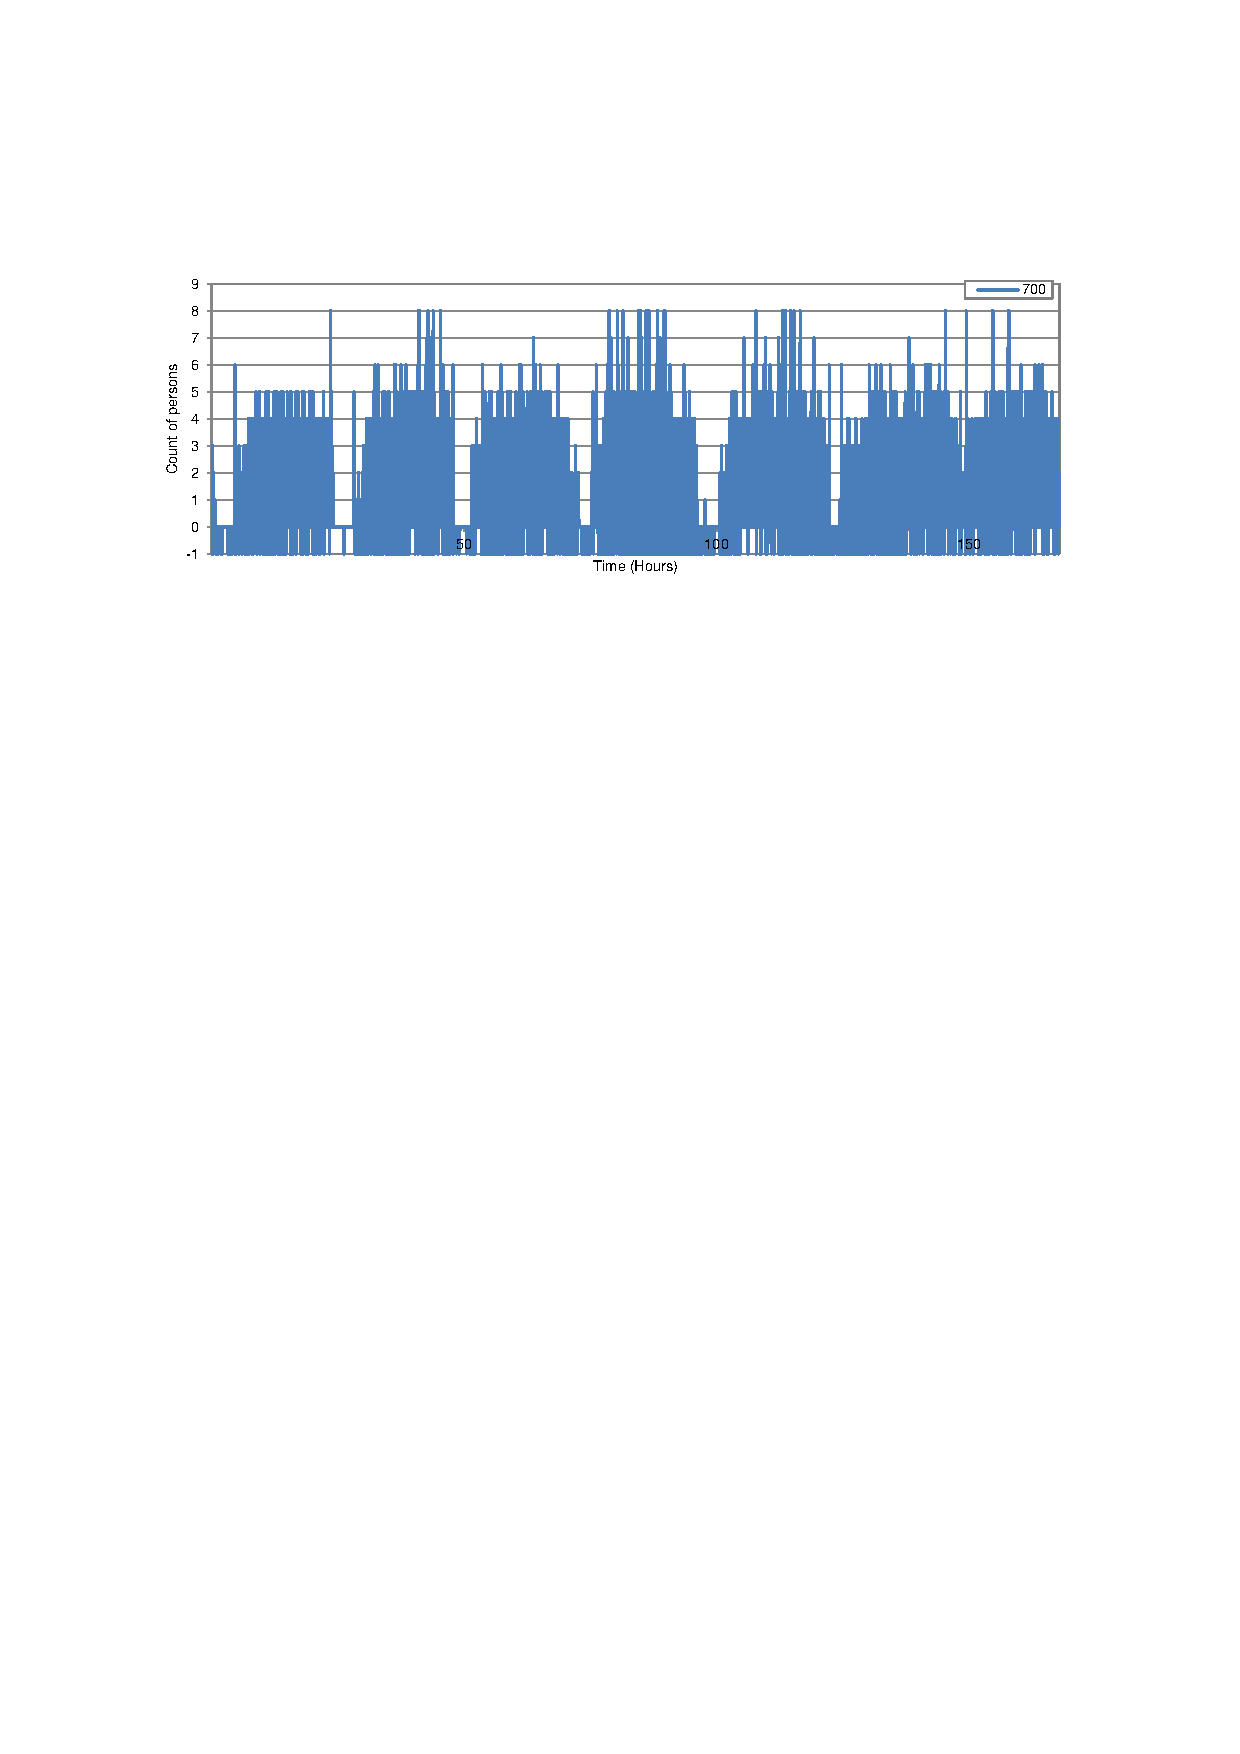
\includegraphics[width=0.46\textwidth]{Figures/rawData_week.pdf}
    \label{fig:rawData_week}
  }
  \hfill
  \subfigure[Passenger density distribution of one camera during one day.] {
    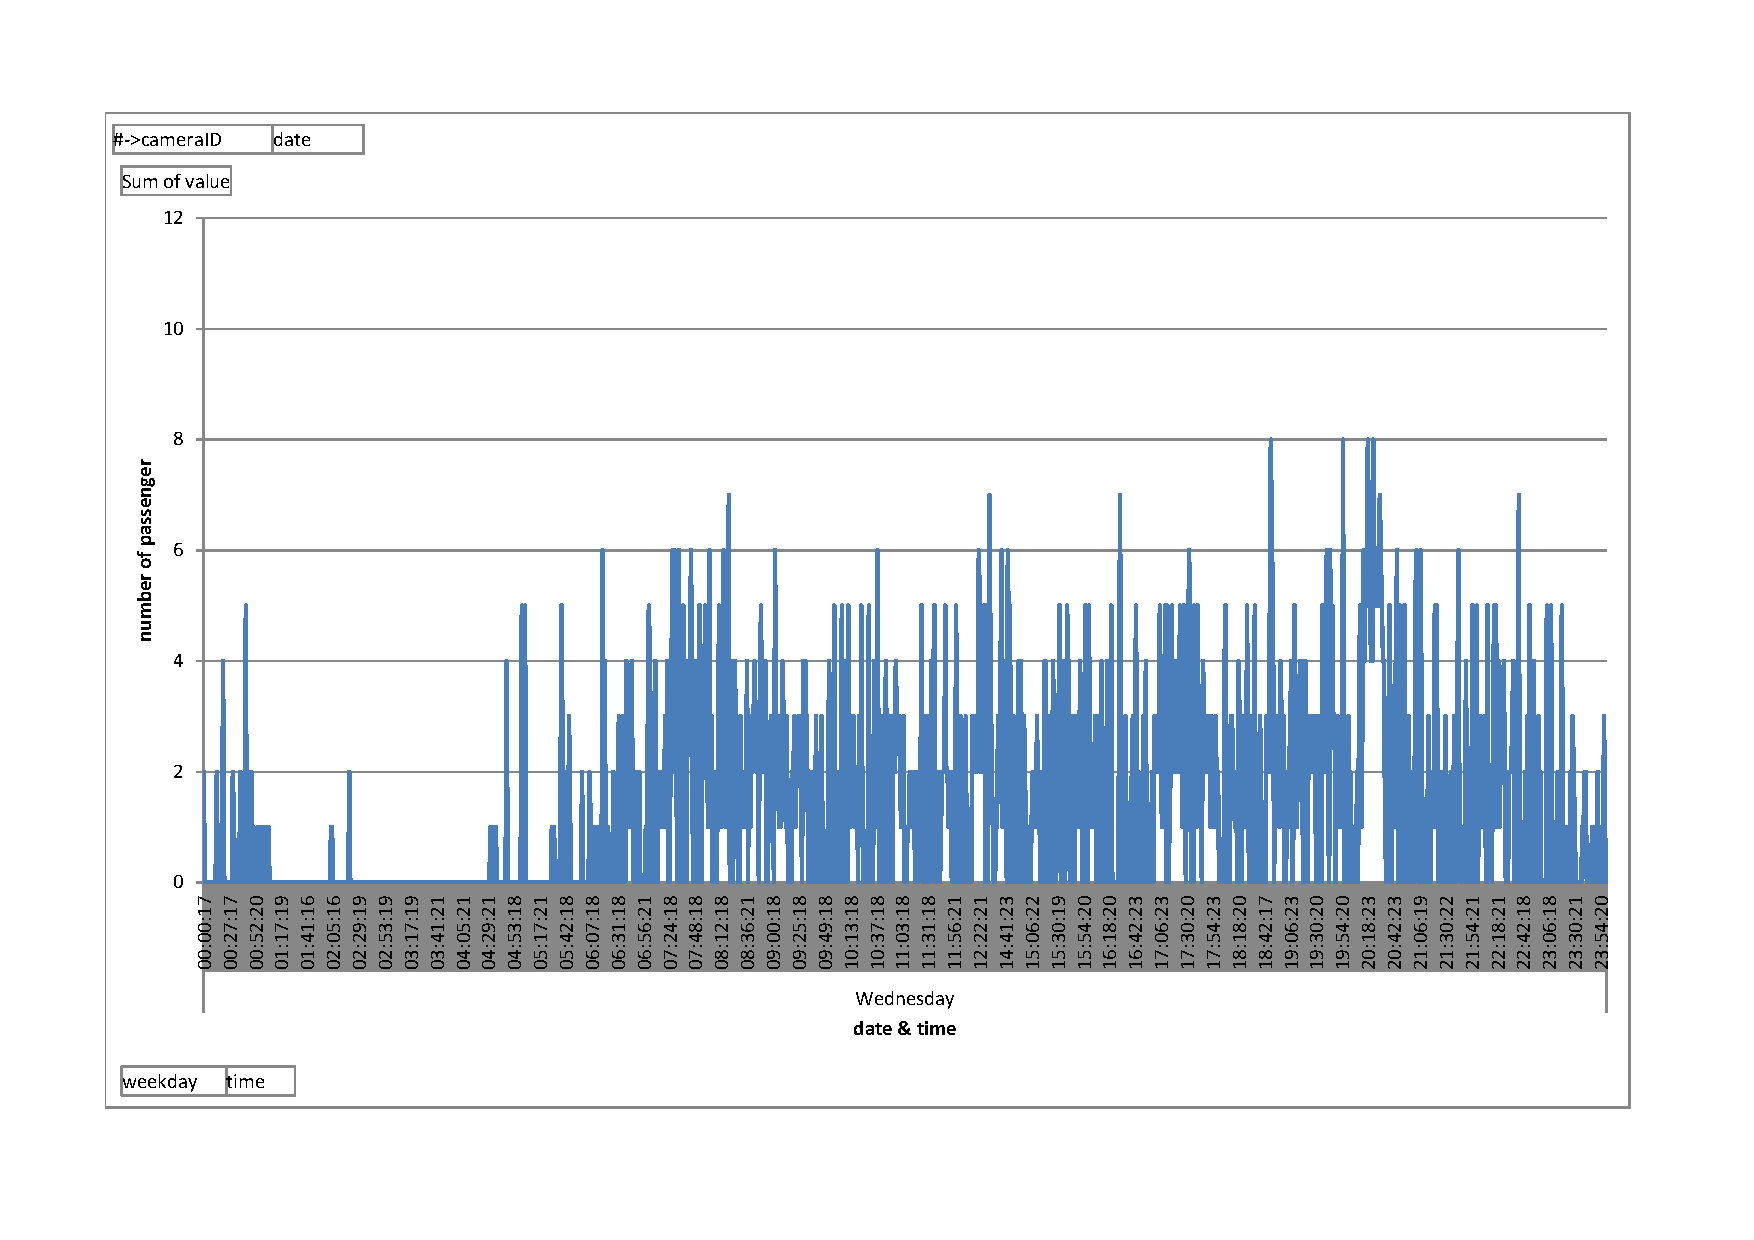
\includegraphics[width=0.46\textwidth]{Figures/rawData_day.pdf}
    \label{fig:rawData_day}
  }

  \caption{Passenger density distribution of one CCTV camera in PdG-L3.}
  \label{fig:rawData}

\end{figure*}